\documentclass[../main.tex]{subfiles}
\begin{document}
\chapter{Recurrence Relations}
As we mentioned briefly about the power of recursion is in the whole algorithm design and analysis, we dedicate this chapter to recurrence relation. To summarize, recurrence relation can help with:
\begin{itemize}
    \item Recurrence relation naturally represent the relation of recursion. Examples will be shown in Chapter.~\ref{chapter_divide_conquer}.
    \item Any iteration can be translated into recurrence relation. Some examples can be found in Chapter.~\ref{chapter_complexity_analysis}.
    \item Recurrence relation together with mathematical induction is the most powerful tool to \textbf{design} and \textbf{prove} the correctness of algorithm(chapter.~\ref{chapter_divide_conquer} and Chapter.~\ref{chapter_complexity_analysis}).
    \item Recurrence relation can be applied to algorithm complexity analysis( Chapter.~\ref{chapter_complexity_analysis}).
\end{itemize}

In  the following chapters of this part, we endow application meanings to these formulas and discuss how to realize the mentioned uses. 

\section{Introduction}
\paragraph{Definition and Concepts} A recurrence relation is  function expressed with the same function. More precisely, as defined in mathematics, recurrence relation is an equation that recursively defines a sequence or multidimensional array of values; once one or more initial terms are given, each further term of the sequence or array is defined as a function of the preceding terms. Fibonacci sequence is one of the most famous recurrence relation which is defined as $f(n)=f(n-1)+f(n-2), f(0)=0, f(1)=1$.
\begin{equation}
    a_n = \Psi(n, a_{n-1})  \text{ for $n \leq 0$,}
\end{equation}

We use $a_n$ to denote the value at index $n$, and the recurrence function is marked as $\Psi(n, P)$, $P$ is all preceding terms that needed to build up this recurrence relation. Like the case of factorial, each factorial number only relies on the result of the previous number and its current index, this recurrence relation can be written as the following equation: 

A recurrence relation needs to start from \textit{initial value(s)}. For the above relation, $a_0$ needs to be defined and it will be the first element of a recurrence relation. The above relation is only related to the very first preceding terms, which is called recurrence relation of \textit{first order}. If $P$ includes multiple preceding terms, a recurrence relation of order $k$ can be easily extended as:
\begin{equation}
    a_n = \Psi(n, a_{n-1}, a_{n-2}, ..., a_{n-k})  \text{ for $n \leq k$,}
\end{equation}
In this case, $k$ initial values are needed for defining a sequence. Initial values can be given any values but then once initial values are decided,  the recurrence determines the sequence uniquely. Thus, initial values are also called the \textit{degree of freedom} for solutions to the recurrence. 

Many natural functions are easily expressed as recurrence:
\begin{itemize}
    \item Polynomial: $a_n = a_{n-1}+1, a_1=1 \xrightarrow{} a_n = n$.
    \item Exponential: $a_n = 2 \times a_{n-1}, a_1=1 \xrightarrow{} a_n = 2^{n-1}$.
    \item Factorial: $a_n = n\times a_{n-1}, a_1=1 \xrightarrow{}a_n = n!$
\end{itemize}

\paragraph{Solving Recurrence Relation} In real problems, we might care about the value of recursion at $n$, that is compute $a_n$ for any given $n$, and there are two ways to do it: 
\begin{itemize}
    \item Programming: we utilize the computational power of computer and code in either iteration or recursion to build up the value at any given $n$. For example, $f(2)=f(1)+f(0)=1$, $f(3)=f(2)+f(1)=2$, and so on. With this iteration, we would need $n-1$ steps to compute $f(n)$. 
    \item Math: we solve the recurrence relation by obtaining an explicit or closed-form expression which is a non-recursive function of $n$. With the solution at hand, we can get  $a_n$ right away.
\end{itemize}
 Recurrence relations plays an important role in the analysis of algorithms. Usually, time recurrence relation $T(n)$ is defined to analyze the time complexity of solving a problem with input instance of size $n$. The field of complexity analysis studies the closed-form solution of $T(n)$; that is to say the functional relation between $T(n)$ with $n$ that it cares, not each exact value. 
 
 
In this section, we focus on solving the recurrence relation using math to get a closed-form solution.  Categorizing the recurrence relation can help us pinpoint each type's solving methods. 

\paragraph{Categorizes} Recurrence relation is essentially discreet function, which can be naturally categorized as \textbf{linear} (such as function $y=mx+b)$ and \textbf{non-linear}; quadratic, cubic and so on (such as $y=ax^2+bx+c, y=ax^3+bx^2+cx+d$). In the field of algorithmic problem solving, linear recurrence relation is commonly used and researched, thus we deliberately leave the non-linear recurrence relation and its method of solving out of the scope of this book. 
% \begin{itemize}
%     \item Linear Recurrence Relation: 
    \begin{itemize}
        \item \textbf{Homogeneous linear recurrence relation:} When the recurrent relation is linear homogeneous of degree $k$ with constant coefficients, it is in the form, and is also called order-k homogeneous linear recurrence with constant coefficients. 
        \begin{equation}
            a_n=c_1a_{n-1} + c_2a_{n-2} + ... + c_k a_{n-k}.
            \label{eq_homogeneous_recurrence_relation}
        \end{equation}
        $a_0, a_1, ..., a_{k-1}$ will be initial values.
 
        \item \textbf{Non-homogeneous linear recurrence relation:} An order-k non-homogeneous linear recurrence with constant coefficients is defined in the form:
                \begin{equation}
            a_n=c_1a_{n-1} + c_2a_{n-2} + ... + c_k a_{n-k}+f(n).
             \label{eq_non_homogeneous_recurrence_relation}
        \end{equation}
        f(n) can be 1 or $n$ or $n^2$ and so on. 
        \item \textbf{Divide-and-conquer recurrence relation}: When $n$ is not decreasing by a constant as does in Eq.~\ref{eq_homogeneous_recurrence_relation} and Eq.~\ref{eq_non_homogeneous_recurrence_relation}, instead by a constant factor, with the equality as shown below, it is called divide and conquer recurrence relation. 
        \begin{equation}
    a_n=a_{n/b}+f(n)
    \label{divide_conquer_eq1}
\end{equation}
where $a\leq 1, b>1$, and $f(n)$ is a given function, which usually has $f(n)= cn^k$. 
%The special method for solving divide and conquer which is named \textit{master method} will be introduced in Chapter.~\ref{chapter_divide_conquer} when we have enough understanding of the term--divide and conquer. 
        
    \end{itemize}
%     \item Non-linear Recurrence Relation
% \end{itemize}
We will introduce general methods to solve a linear recurrence relation but leave out the part of divide and conquer recurrence relation in this chapter for reason that divide and conquer recurrence relation will most likely to be solved with just roughly, as shown in Chapter.~\ref{chapter_complexity_analysis} to just estimate the time complexity resulted from the divide and conquer method. 

\section{General Methods to Solve Linear Recurrence Relation}
 No general method for solving recurrence function is known yet, however, linear recurrence relation with finite initial values and previous states, constant coefficients can always be solved. Due to the fact that the recursion is essentially mathematical induction, the most general way of solving any recurrence relation is to use \textit{mathematical induction} and \textit{iterative method}. This also makes the the mathematical induction, in some form, the foundation of all correctness proofs for computer programs.  We  examine these two methods by solving two recurrence relation: $a_n = 2\times a_{n-1} + 1, a_0 = 0$ and $a_n=a_{n/2} + 1$. 

\subsection{Iterative Method}
The most straightforward method for solving recurrence relation no matter its linear or non-linear is the \textit{iterative method}. Iterative method is a technique or procedure in computational mathematics that it iteratively replace/substitute each $a_n$ with its recurrence relation $\Psi(n, a_{n-1}, a_{n-2}, ..., a_{n-k})$ till all items ``disappear'' other than the initial values. Iterative method is also called substitution method. 

We demonstrate iteration with a simple non-overlapping recursion. 
\begin{align}
\label{complexity_eq_binary_search}
    T(n)&=T(n/2)+O(1)\\
    &=T(n/2^2)+O(1)+O(1)\notag\\
    &=T(n/2^3)+3O(1)\notag\\
    &=...\notag\\
    &=T(1)+kO(1)
\end{align}
We have $\frac{n}{2^k}=1$, we solve this equation and will get $k=\log_2 n$. Most likely $T(1)=O(1)$ will be the initial condition, we replace this, and we get $T(n)=O(\log_2 n)$.

However, when we try to apply iteration on the third recursion:  $T(n)=3T(n/4)+O(n)$. It might be tempting to assume that $T(n)=O(n\log n)$ due to the fact that $T(n)=2T(n/2)+O(n)$ leads to this time complexity.
\begin{align}
\label{complexity_non_overlap_1}
    T(n)&=3T(n/4)+O(n)\\
    &=3(3T(n/4^2)+n/4)+n=3^2T(n/4^2)+n(1+3/4)\notag\\
    &=3^2(3T(n/4^3)+n/4^2)+n(1+3/4)=3^3T(n/4^3)+n(1+3/4+3/4^2)\\
    &=...\\
    &=3^kT(n/4^k)+n\sum_{i=0}^{k-1}(\frac{3}{4})^{i}
\end{align}
\subsection{Recursion Tree}
Since the term of T(n) grows, the iteration can look messy. We can use recursion tree to better visualize the process of iteration. In a recursive tree, each node represents the value of a single subproblem, and a leaf would be a subproblem. As a start, we expand $T(n)$ as a node with value $n$ as root, and it would have three children each represents a subproblem $T(n/4)$. We further do the same with each leaf node, until the subproblem is trivial and be a base case. In practice, we just need to draw a few layers to find the rule. The cost will be the sum of costs of all layers.  The process can be seen in  Fig.~\ref{fig:recursive_tree}. 
\begin{figure}[!ht]
    \centering
    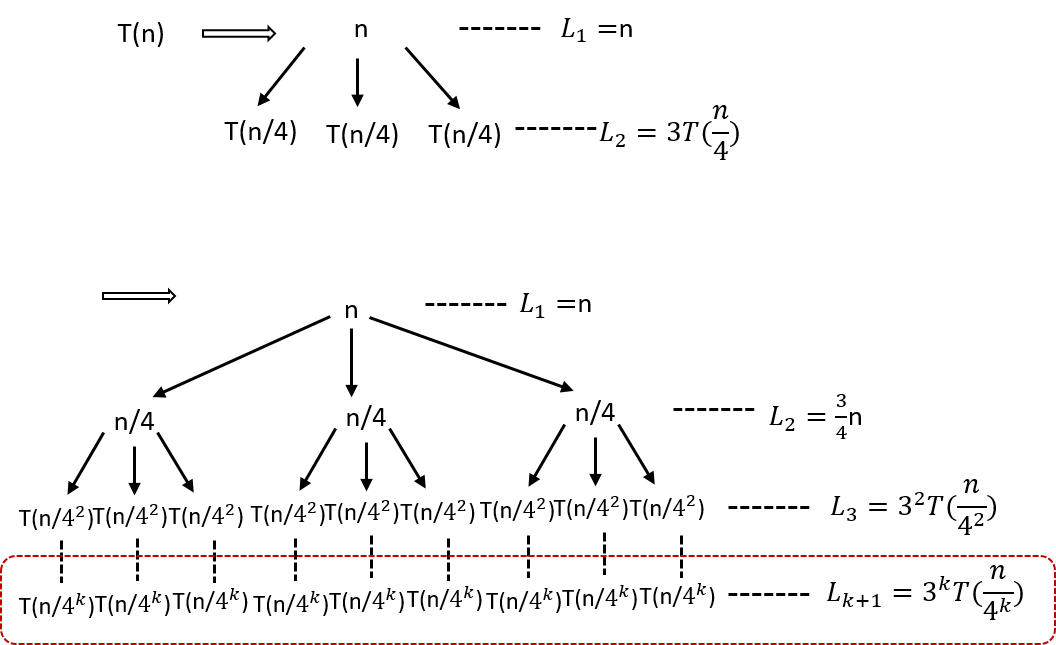
\includegraphics[width=0.98\columnwidth]{fig/recursion_tree_non_overlap.png}
    \caption{The process to construct a recursive tree for $T(n) = 3T(\floor*{n/4}) + O(n)$. There are totally k+1 levels. Use a better figure.  }
    \label{fig:recursive_tree}
\end{figure}
 In this case, it is the base case $T(1)$. Through the expansion with iteration and recursion tree, our time complexity function becomes:
\begin{align}
\label{complexity_non_overlap_2}
    T(n)&=\sum_{i=1}^{k}L_i + L_{k+1}\\
    &=n\sum_{i=1}^{k}(3/4)^{i-1}+3^kT(n/4^k)
\end{align}

In the process, we can see that Eq.~\ref{complexity_non_overlap_2} and Eq.~\ref{complexity_non_overlap_1} are the same.  Because $T(n/4^k)=T(1)=1$, we have $k=\log_4 n$. 
\begin{align}
\label{complexity_non_overlap_2}
    T(n)&\leq n\sum_{i=1}^{\infty}(3/4)^{k-1}+3^kT(n/4^k)\\
    &\leq 1/(1-3/4)n+3^{\log_4 n} T(1)= 4n+n^{log_4 3}
    &\leq 5n \\
    &=O(n)
\end{align}



\subsection{Mathematical Induction}
Mathematical induction is a mathematical proof technique, and is essentially used to prove that a property $P(n)$ holds for every natural number $n$, i.e. for $n=0, 1, 2, 3$, and so on. Therefore, in order to use induction, we need to make a \textit{guess} of the closed-form solution for $a_n$. Induction requires two cases to be proved. 
\begin{enumerate}
    \item 
 \textit{Base case:} proves that the property holds for the number $0$. 
\item \textit{Induction step:} proves that, if the property holds for one natural number $n$, then it holds for the next natural number $n+1$.
\end{enumerate}

For $T(n)=2\times T(n-1) +1, T_0 = 0$, we can have the following result by expanding $T(i), i \in [0, 7]$.
\begin{lstlisting}[numbers=none]
n    0 1 2 3 4 5 6 7
T_n  0 3 7 15 31 63 127
\end{lstlisting}
It is not hard that we find the rule and guess $T(n) = 2^n-1$. Now, we prove this equation by induction:
\begin{enumerate}
    \item Show that the basis is true: $T(0) = 2^0 -1 = 0$.
    \item Assume it holds true for $T(n-1)$. By induction, we get
    \begin{align}
        T(n)&=2T(n-1) + 1 \\
        &=2 (2^{n-1} - 1) + 1 \\
        &= 2^n -1
    \end{align}
    Now we show that the induction step holds true too. 
\end{enumerate}

\begin{bclogo}[couleur = blue!30, arrondi=0.1,logo=\bccrayon,ombre=true]{Solve $T(n)=T(n/2)+O(1)$ and $T(2n)\leq2T(n)+2n-1, T(2)=1$.}
\end{bclogo}


\paragraph{Briefying on Other Methods}
When the form of the linear recurrence is more complex, say large degree of $k$, more complex of the $f(n)$, none of the iterative and induction methods is practical and managable. For iterative method, the expansion will be way too messy for us to handle. On the side of induction method, it is quite challenging or sometimes impossible for us just to ``guess'' or ``generalize'' the exact closed-form of recurrence relation solution purely based on observing a range of expansion.   

The more general and approachable method  for solving homogeneous linear recurrence relation derives from making a rough guess rather than exact guess, and then solve it via \textit{characteristic equation}. This general method is pinpointed in Section.~\ref{subsec_homogeneous_linear_recurrence} with examples. For non-homogeneous linear recurrence relation (Section.~\ref{subsec_non_homogeneous}), there are generally two ways -- \textit{symbolic differentiation} and \textit{method of undetermined coefficients} to solve non-homogeneous linear recurrence relation and both of them relates to solving homogeneous linear relation. The study of the remaining content is most math saturated in the book, while we later on will find out its tremendous help in complexity analysis in Chapter.~\ref{chapter_complexity_analysis} and potentially in problem solving. 

% \paragraph{Examples} Maybe

% \subsection{Solving Linear Recursion}
\section{Solve Homogeneous Linear Recurrence Relation}

\label{subsec_homogeneous_linear_recurrence} 
In this section, we offer a more general and more managable method for solving recurrence relation that is homogeneous defined in Eq.~\ref{eq_homogeneous_recurrence_relation}. There are three broad methods: using characteristic equation which we will learn  in this section, and the other two-- {linear algebra, and Z-transofrm}~\footnote{Visit \url{https://en.wikipedia.org/wiki/Recurrence_relation} for details.} will not be included. 
\paragraph{Make a General ``Guess''} From our previous examples, we can figure out the closed-form solution for simplied homogeneous linear recurrence such as the fibonacci recurrence relation:
\begin{equation}
a_n = a_{n-1}+a_{n-2}, a_0=0, a_1=1
\label{homogeneous_linear_recurrence_guess}
\end{equation}
A reasonable guess would be that $a_n$ is doubled every time; namely, it is approximately $2^n$. Let's guess $a_n=c2^n$ for some constant $c$. Now we substitute Eq.~\ref{homogeneous_linear_recurrence_guess}, we get
\begin{equation}
c2^n = c2^{n-1} + c2^{n-2} = c2^n
\label{homogeneous_linear_recurrence_guess}
\end{equation}
We can see that $c$ will be canceled and the left side is always greater than the right side. Thus we learned that $c2^n$ is a too large guess, and the multiplicative constant $c$ plays no role in the induction step. 

Based on the above example, we introduce a parameter $\gamma$ as a base, $a_n = \gamma ^{n}$ for some $\gamma$. We then compute its value through solving \textit{Characteristic Equation} as introduced below. 
\paragraph{Characteristic Equation} 
Now, we substitute our guess into the Eq.\ref{eq_homogeneous_recurrence_relation}, then 
\begin{align}
    \gamma^n & = a_n \\
    &= c_1 \gamma^{n-1} + c_2 \gamma^{n-2} + ... +  c_k \gamma^{n-k}.
    \label{eq_characteristic_equation_1}
\end{align}
We rewrite Eq.~\ref{eq_characteristic_equation_1} as:
\begin{align}
    \gamma^n  - c_1 \gamma^{n-1} - c_2 \gamma^{n-2} - ... -  c_k \gamma^{n-k} = 0.
    \label{eq_characteristic_equation_2}
\end{align}
By dividing $\gamma^{n-k}$ from left and right side of the equation, we get the simplified equation, which is called the \textit{characteristic equation} of the recurrence relation in the form of Eq.~\ref{eq_homogeneous_recurrence_relation}.
\begin{align}
    \gamma^k  - c_1 \gamma^{k-1} - c_2 \gamma^{k-2} - ... -  c_k = 0.
    \label{eq_characteristic_equation_3}
\end{align}
The concept of characteristic equation is related to generating function\footnote{}.  The solutons of characteristic equation are called \textit{characteristic roots}. 

\paragraph{Characteristic Roots and Solution} Now, we have a linear homogeneous recurrence relation and its characteristic equation, 
% \begin{align}
%   a_n&=c_1a_{n-1} + c_2a_{n-2} + ... + c_k a_{n-k}. \\
% 0&= \gamma^k  - c_1 \gamma^{k-1} - c_2 \gamma^{k-2} - ... -  c_k.
% \end{align}
and assume that the equation has $k$ distinct roots, $\gamma_1, \gamma_2, ..., \gamma_k$, then we can build upon these chracteristic roots, the general guess, and some other $k$ constants, $d_1, d_2, ,,, d_k$ of $\{a_n\}$ as:
\begin{align}
    a_n = d_1\gamma_1^n + d_2\gamma_2^n +...+d_k\gamma_k^n
\end{align}
The unknown constants, $d_1, d_2, ,,, d_k$ of $\{a_n\}$ can be found using the initial values $a_0, a_1, ..., a_{k-1}$ by solving the following equations:
\begin{align}
    a_0 &= d_1\gamma_1^0 + d_2\gamma_2^0 +...+d_k\gamma_k^0,\\
    a_1 &= d_1\gamma_1^1 + d_2\gamma_2^1 +...+d_k\gamma_k^1, \\
    &...,\\
    a_{k-1} &= d_1\gamma_1^{k-1} + d_2\gamma_2^{k-1} +...+d_k\gamma_k^{k-1}.
\end{align}
Within the context of computer science, the degree is mostly within 2. Here, we introduce the formula solving the character roots for  characteristic equation with the following form:
\begin{equation}
   0 = ax^2+bx+c
\end{equation}
% The root(s) of the function is the value(s) of $x$ which makes $f(x)=0$. 
The root(s) can be computed from the following formula~\footnote{Visit {http://www.biology.arizona.edu/biomath/tutorials/Quadratic/Roots.html} for derivation} :
\begin{equation}
    x = \frac{-b \pm \sqrt{b^2-4ac}}{2a}
\end{equation}
\paragraph{Hands-on Example}
For $a_n = 2a_{n-1} + 3a_{n-2}, a_0=3, a_1=5$, we can write the characteristic equation as $\gamma^2-2\gamma-3=0$. Because $\gamma^2-2\gamma-3 = (\gamma-3)+(\gamma+1)$, which make the characteristic roots $\gamma_1=3, \gamma_2=-1$. Now our solution has the form:
\begin{align}
    a_n = d_13^n+d_2{(-1)}^{n}
\end{align}
Now, we find the constants via listing the initial values we know:
\begin{align}
    a_0 &= d_13^0+d_2{(-1)}^{0} = d_1+d_2=3, \\
 a_1 &= d_13^1+d_2{(-1)}^{1} = 3d_1-d_2=5.
\end{align}
We would get $d_1=2, d_2=1$. Finally, we have a solution $a_n = 2*3^n+(-1)^n$. 
% \paragraph{Linear Algebra}
% \paragraph{Z-transform}
\begin{bclogo}[couleur = blue!30, arrondi=0.1,logo=\bccrayon,ombre=true]{Continue to solve $a_n=a_{n-1}+a_{n-2}$.}
\end{bclogo}

\section{Solve Non-homogeneous Linear Recurrence Relation}
\label{subsec_non_homogeneous}
 \textit{method of undetermined coefficients} where the solution is comprised of the solution of the homogeneous part and the particular $f(n)$ part by summing up; and the method of \textit{symbolic differentiation} which converts from the equation the same form of homogeneous linear recurrence relation. 
 
The complexity analysis for most algorithms fall into the form of non-homogeneous linear recurrence relation. For examples: in fibonacci sequence, if it is be solved by using recursion shown in Chapter.~\ref{chapter_dynamic-programming} without caching mechanism, the time recurrence relation is $T(n)=T(n-1)+T(n-2)+1$; in the merge sort discussed in Chapter.~\ref{chapter_divide_conquer}, the recurrence relation is $T(n)=T(n/2)+n$. Examples of recurrence relation $T(n)=T(n-1)+n$ can be easily found, such as the maximum subarray. 
% \subsection{Solving None-linear Recursion}

\paragraph{Method of Undetermined Coefficients} Suppose we have a recurrence relation in the form of Eq.~\ref{eq_non_homogeneous_recurrence_relation}. 

Suppose we ignore the non-linear part and just look at the homogeneous part:
\begin{equation}
    h_n=c_1h_{n-1} + c_2h_{n-2} + ... + c_k h_{n-k}.
    \label{eq_non_homogeneous_recurrence_relation_2}
\end{equation}

\paragraph{Symbolic Differentiation}



% \section{Hands-on Examples}
% \label{sec_iter_recur_examples}
\section{Useful Math Formulas}
Knowing these facts can be very important in practice, we can treat each as an element in the problem solving. Sometimes, when its hard to get the closed form of a recurrence relation or finding the recurrence relation, we decompse it to multiple parts with these elements. Put some examples. 
\paragraph{binomial theorem}
\begin{align}
    \sum_{k=0}^{n}C_{n}^{k}x^k = (1+x)^n
\end{align}
An example of using this the cost of generating a powerset, where $x=1$.
\section{Exercises}
\begin{enumerate}
    \item Compute factorial sequence using \texttt{while} loop.
    \item Greatest common divisor: The Euclidean algorithm, which computes the greatest common divisor of two integers, can be written recursively.
    \begin{equation}
            gcd(x, y)=
        \begin{cases}
  x & \text{if $y=0$,}\\
  gcd(y, x\% y) & \text{if $y>0$}
\end{cases}
    \end{equation}

Function definition: 
\end{enumerate}

\section{Summary}
If a cursive algorithm can be further optimized, the optimization method can either be divide and conquer or decrease and conquer. We have put much effort into solving recurrence relation of both: the linear recurrence relation for decrease and conquer, the divide and conquer recurrence relation for divide and conquer.  Right now, do not struggle and eager to know what is divide or decrease and conquer, it will be explained in the next two chapters. 

Further, Akra-Bazzi Method~\footnote{} applies to recurrence such that $T(n)=T(n/3)+T(2n/3)+O(n)$. Please look into more details if interested. Generating function is used to solve the linear recurrence.
\end{document}